% =============================================================================
% Chapitre 7 — Démonstrateur, explicabilité et préparation industrielle
% =============================================================================

\chapter{Démonstrateur, explicabilité et préparation industrielle}
\label{chap:demonstrateur}

Le résultat scientifique n'est qu'une partie du livrable. EURAFRIC Information
conçoit des systèmes pour des institutions où une analyse doit être comprise,
versionnée, contrôlée et exposée à plusieurs publics sans divergence. Le projet
a donc été mené comme un petit produit de recherche : un même ensemble
d'artefacts alimente le rapport, le tableau de bord, l'interface REST, les cartes
de modèle et les contrôles de monitoring.

\begin{figure}[htbp]
  \centering
  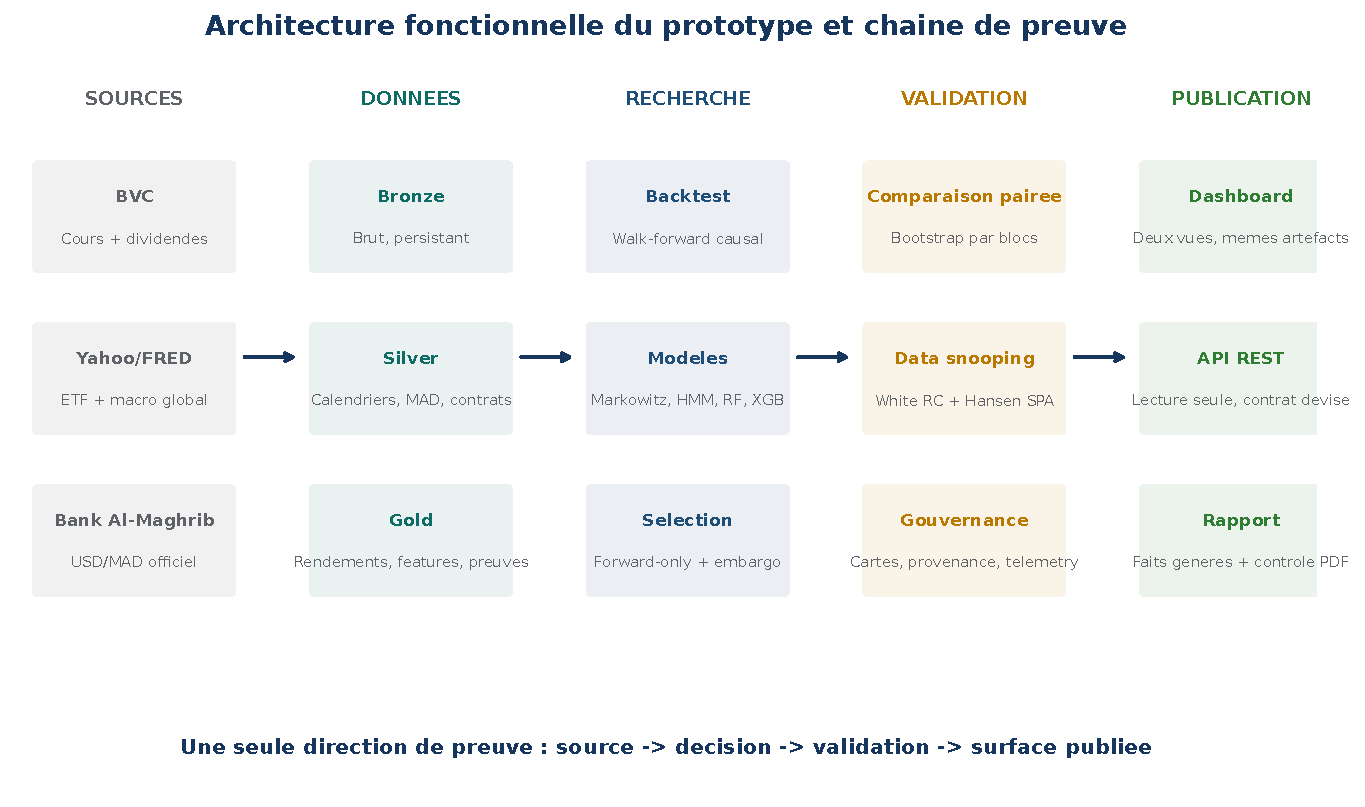
\includegraphics[width=\textwidth]{assets/figures/architecture_globale.pdf}
  \caption{Architecture fonctionnelle du prototype. Les flèches représentent
  une direction de preuve : toute information publiée doit remonter à un
  artefact validé, puis à une transformation et à une source.}
  \label{fig:architecture-finale}
\end{figure}

% -----------------------------------------------------------------------------
\section{Deux interfaces, un seul contrat de vérité}
% -----------------------------------------------------------------------------

La première page du tableau de bord, « Résultats de recherche », s'adresse au
décideur. Elle commence par le numéraire et les limites d'usage, puis présente
le verdict principal, les fenêtres de crise et la force de preuve. Elle ne
présente plus une promesse de valeur ML : les écarts observés sont négatifs sur
les deux univers et aucune surperformance des challengers n'est établie après
correction de la recherche.

\begin{figure}[p]
  \centering
  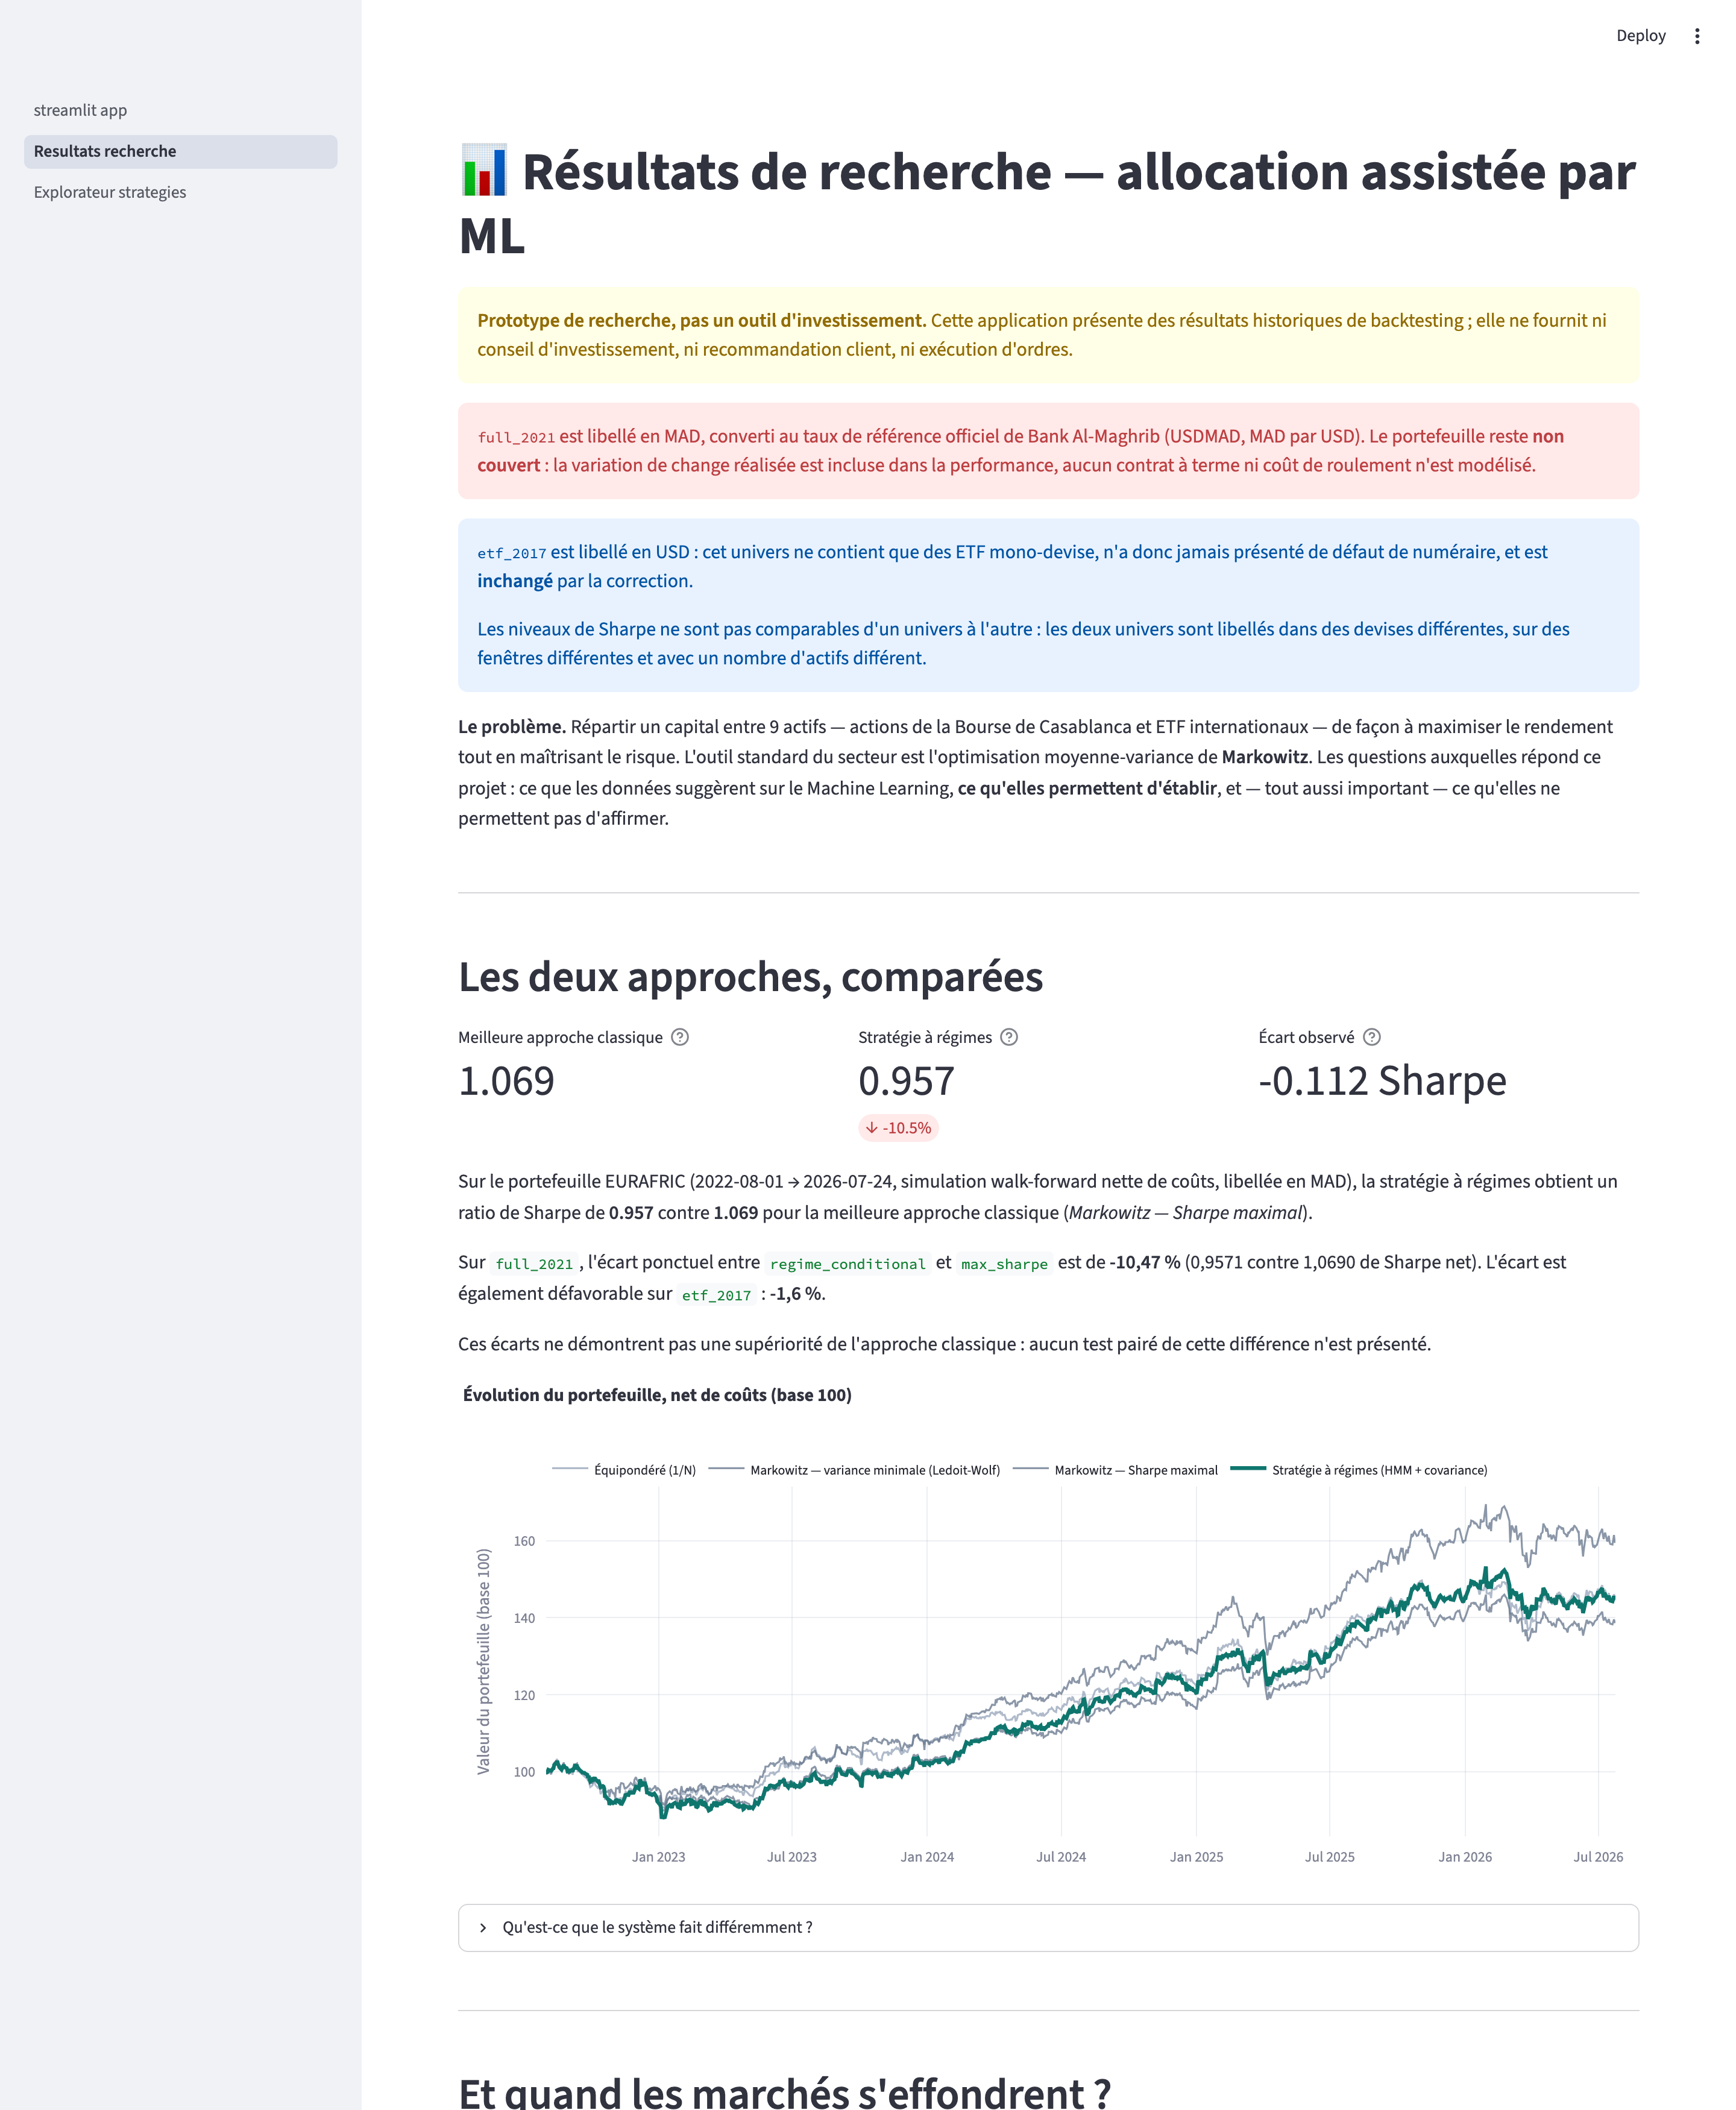
\includegraphics[width=0.94\textwidth]{assets/figures/dashboard_page1_full_01.png}
  \caption{Tableau de bord — page « Résultats de recherche », vue générale.
  Le numéraire MAD, le caractère non couvert et l'écart observé sont visibles
  avant tout détail de stratégie.}
  \label{fig:dashboard-decision}
\end{figure}

\begin{figure}[p]
  \centering
  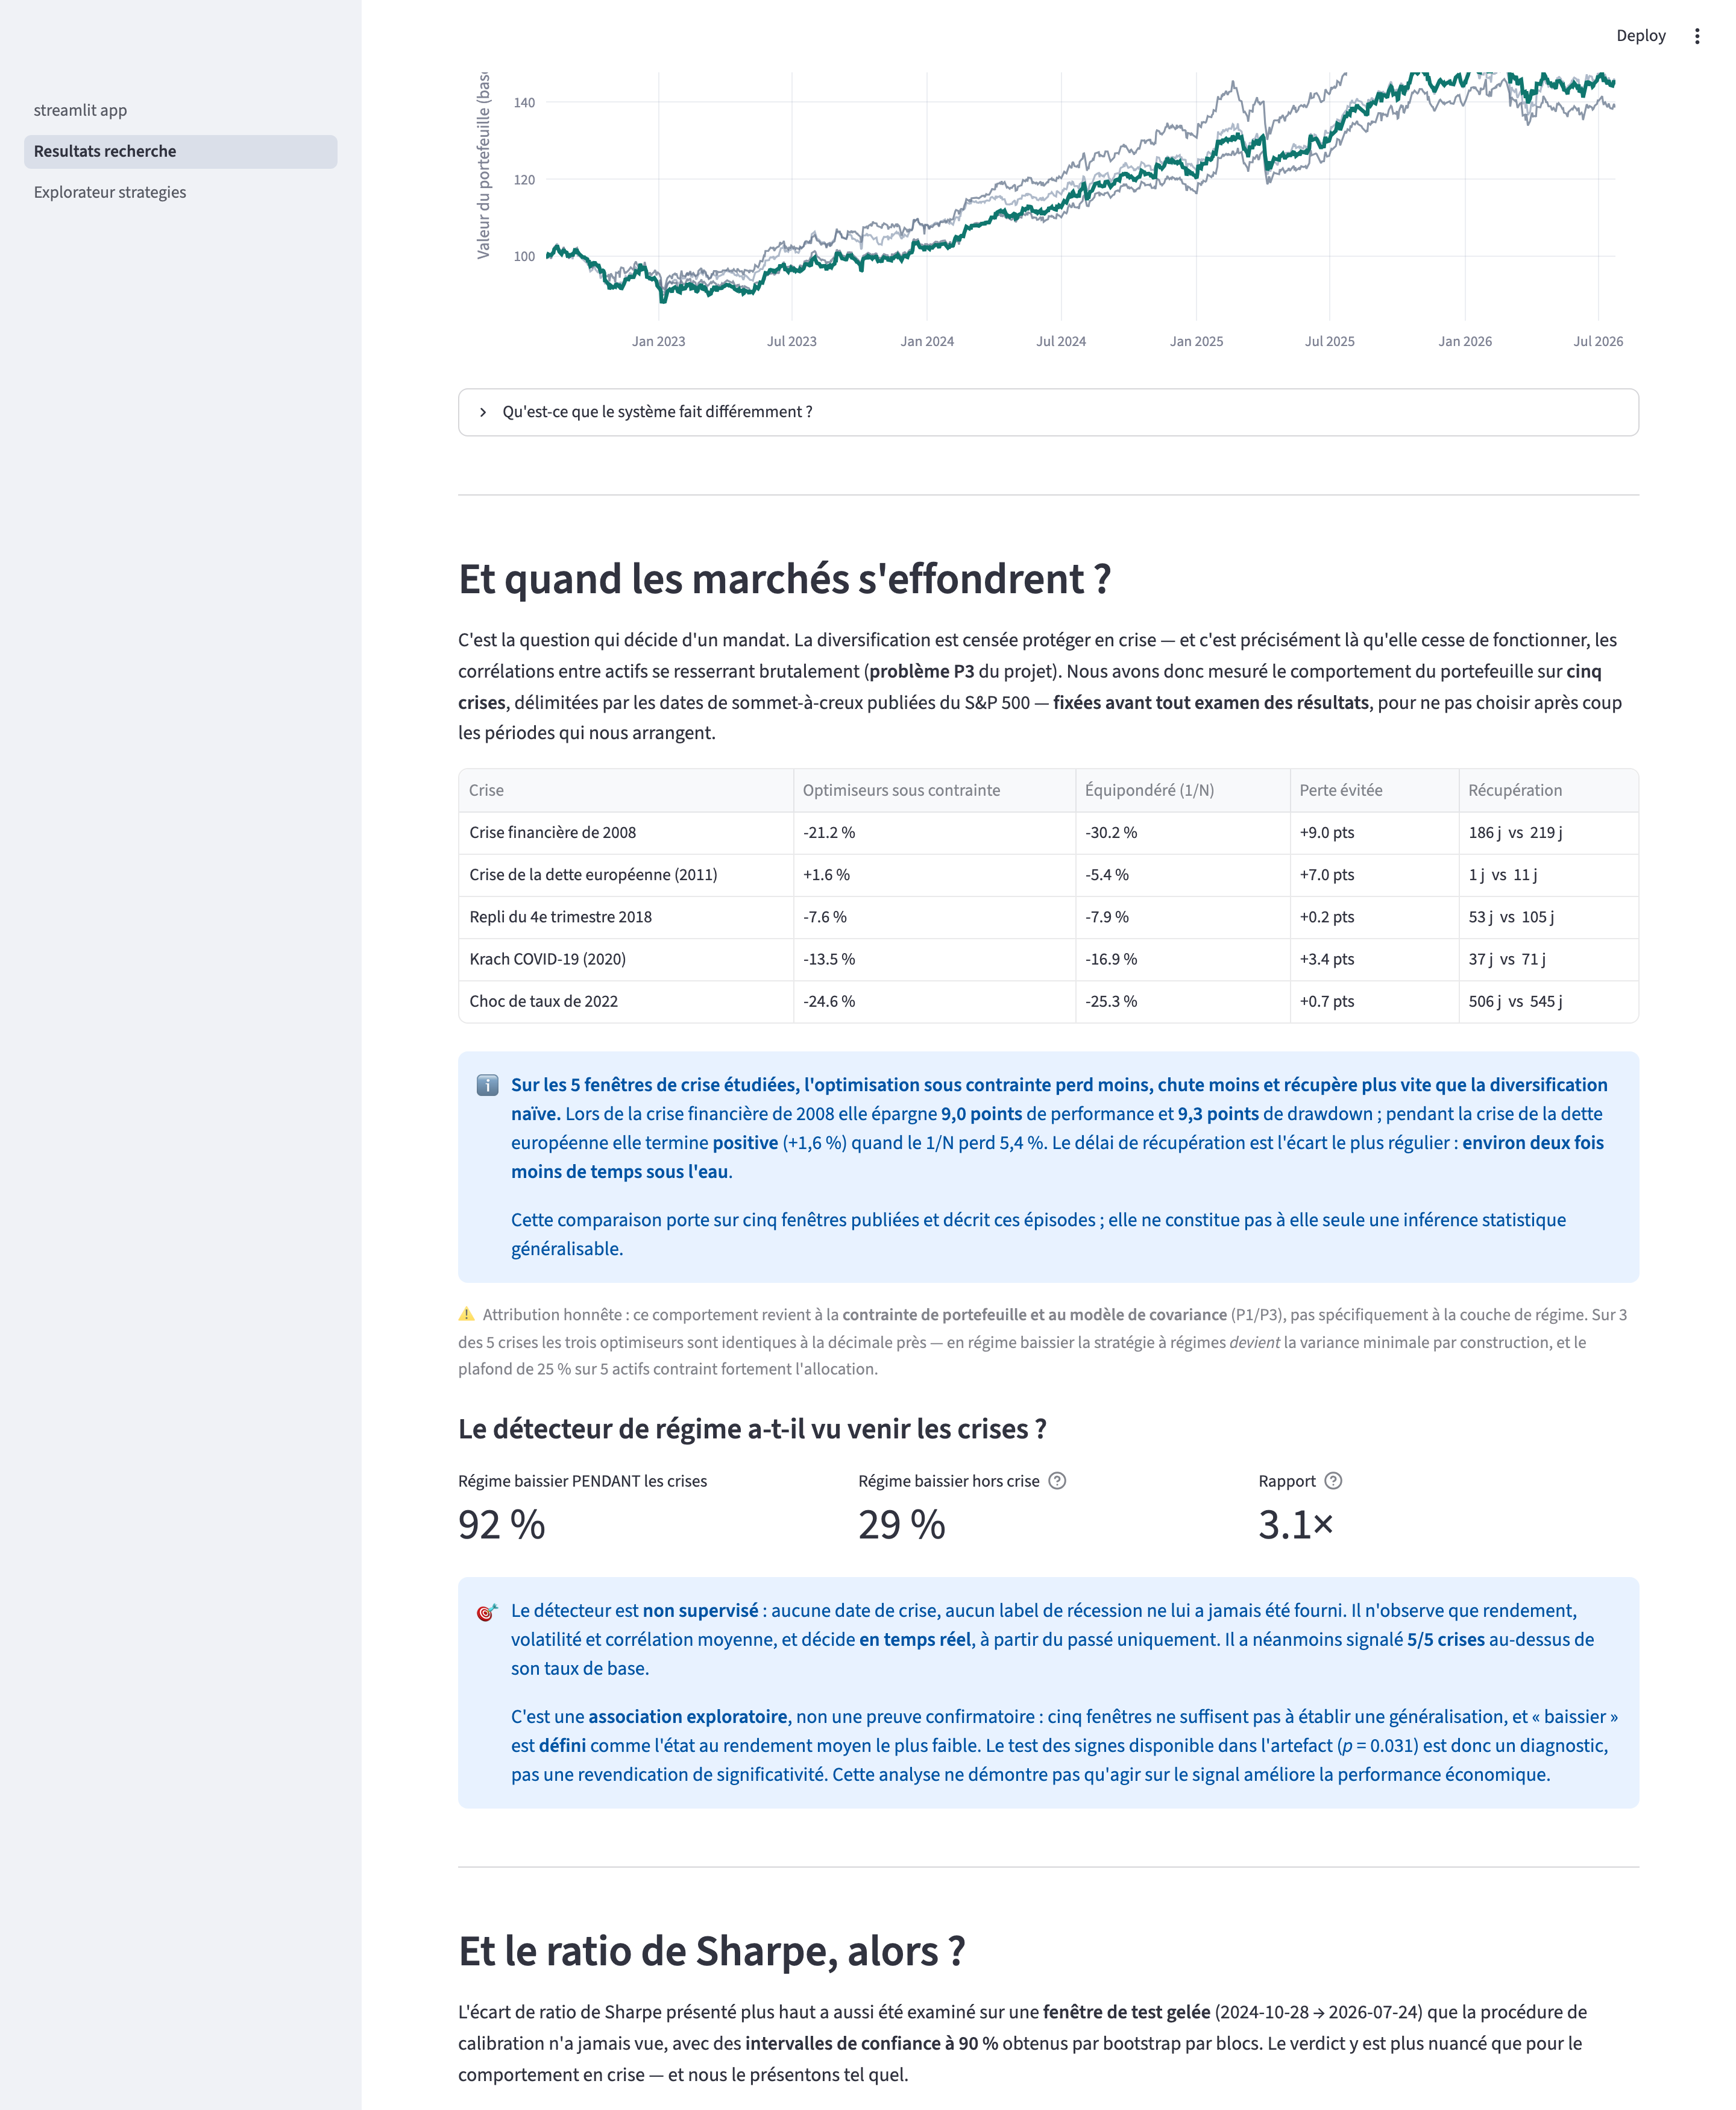
\includegraphics[width=0.94\textwidth]{assets/figures/dashboard_page1_full_02.png}
  \caption{Tableau de bord — attribution des résultats et comportement dans les
  fenêtres de crise. Les diagnostics exploratoires sont séparés des preuves
  confirmatoires.}
  \label{fig:dashboard-crises}
\end{figure}

La seconde page, « Explorateur de stratégies », s'adresse à l'analyste. Elle
permet de filtrer l'univers, la stratégie et les métriques, d'observer la
trajectoire de richesse, les pertes maximales, les allocations et la rotation.
Les deux pages utilisent la même couche de lecture. Un test interdit les ratios
de Sharpe écrits en dur dans le code d'interface : une nouvelle release change
les deux vues ensemble ou échoue.

\begin{figure}[p]
  \centering
  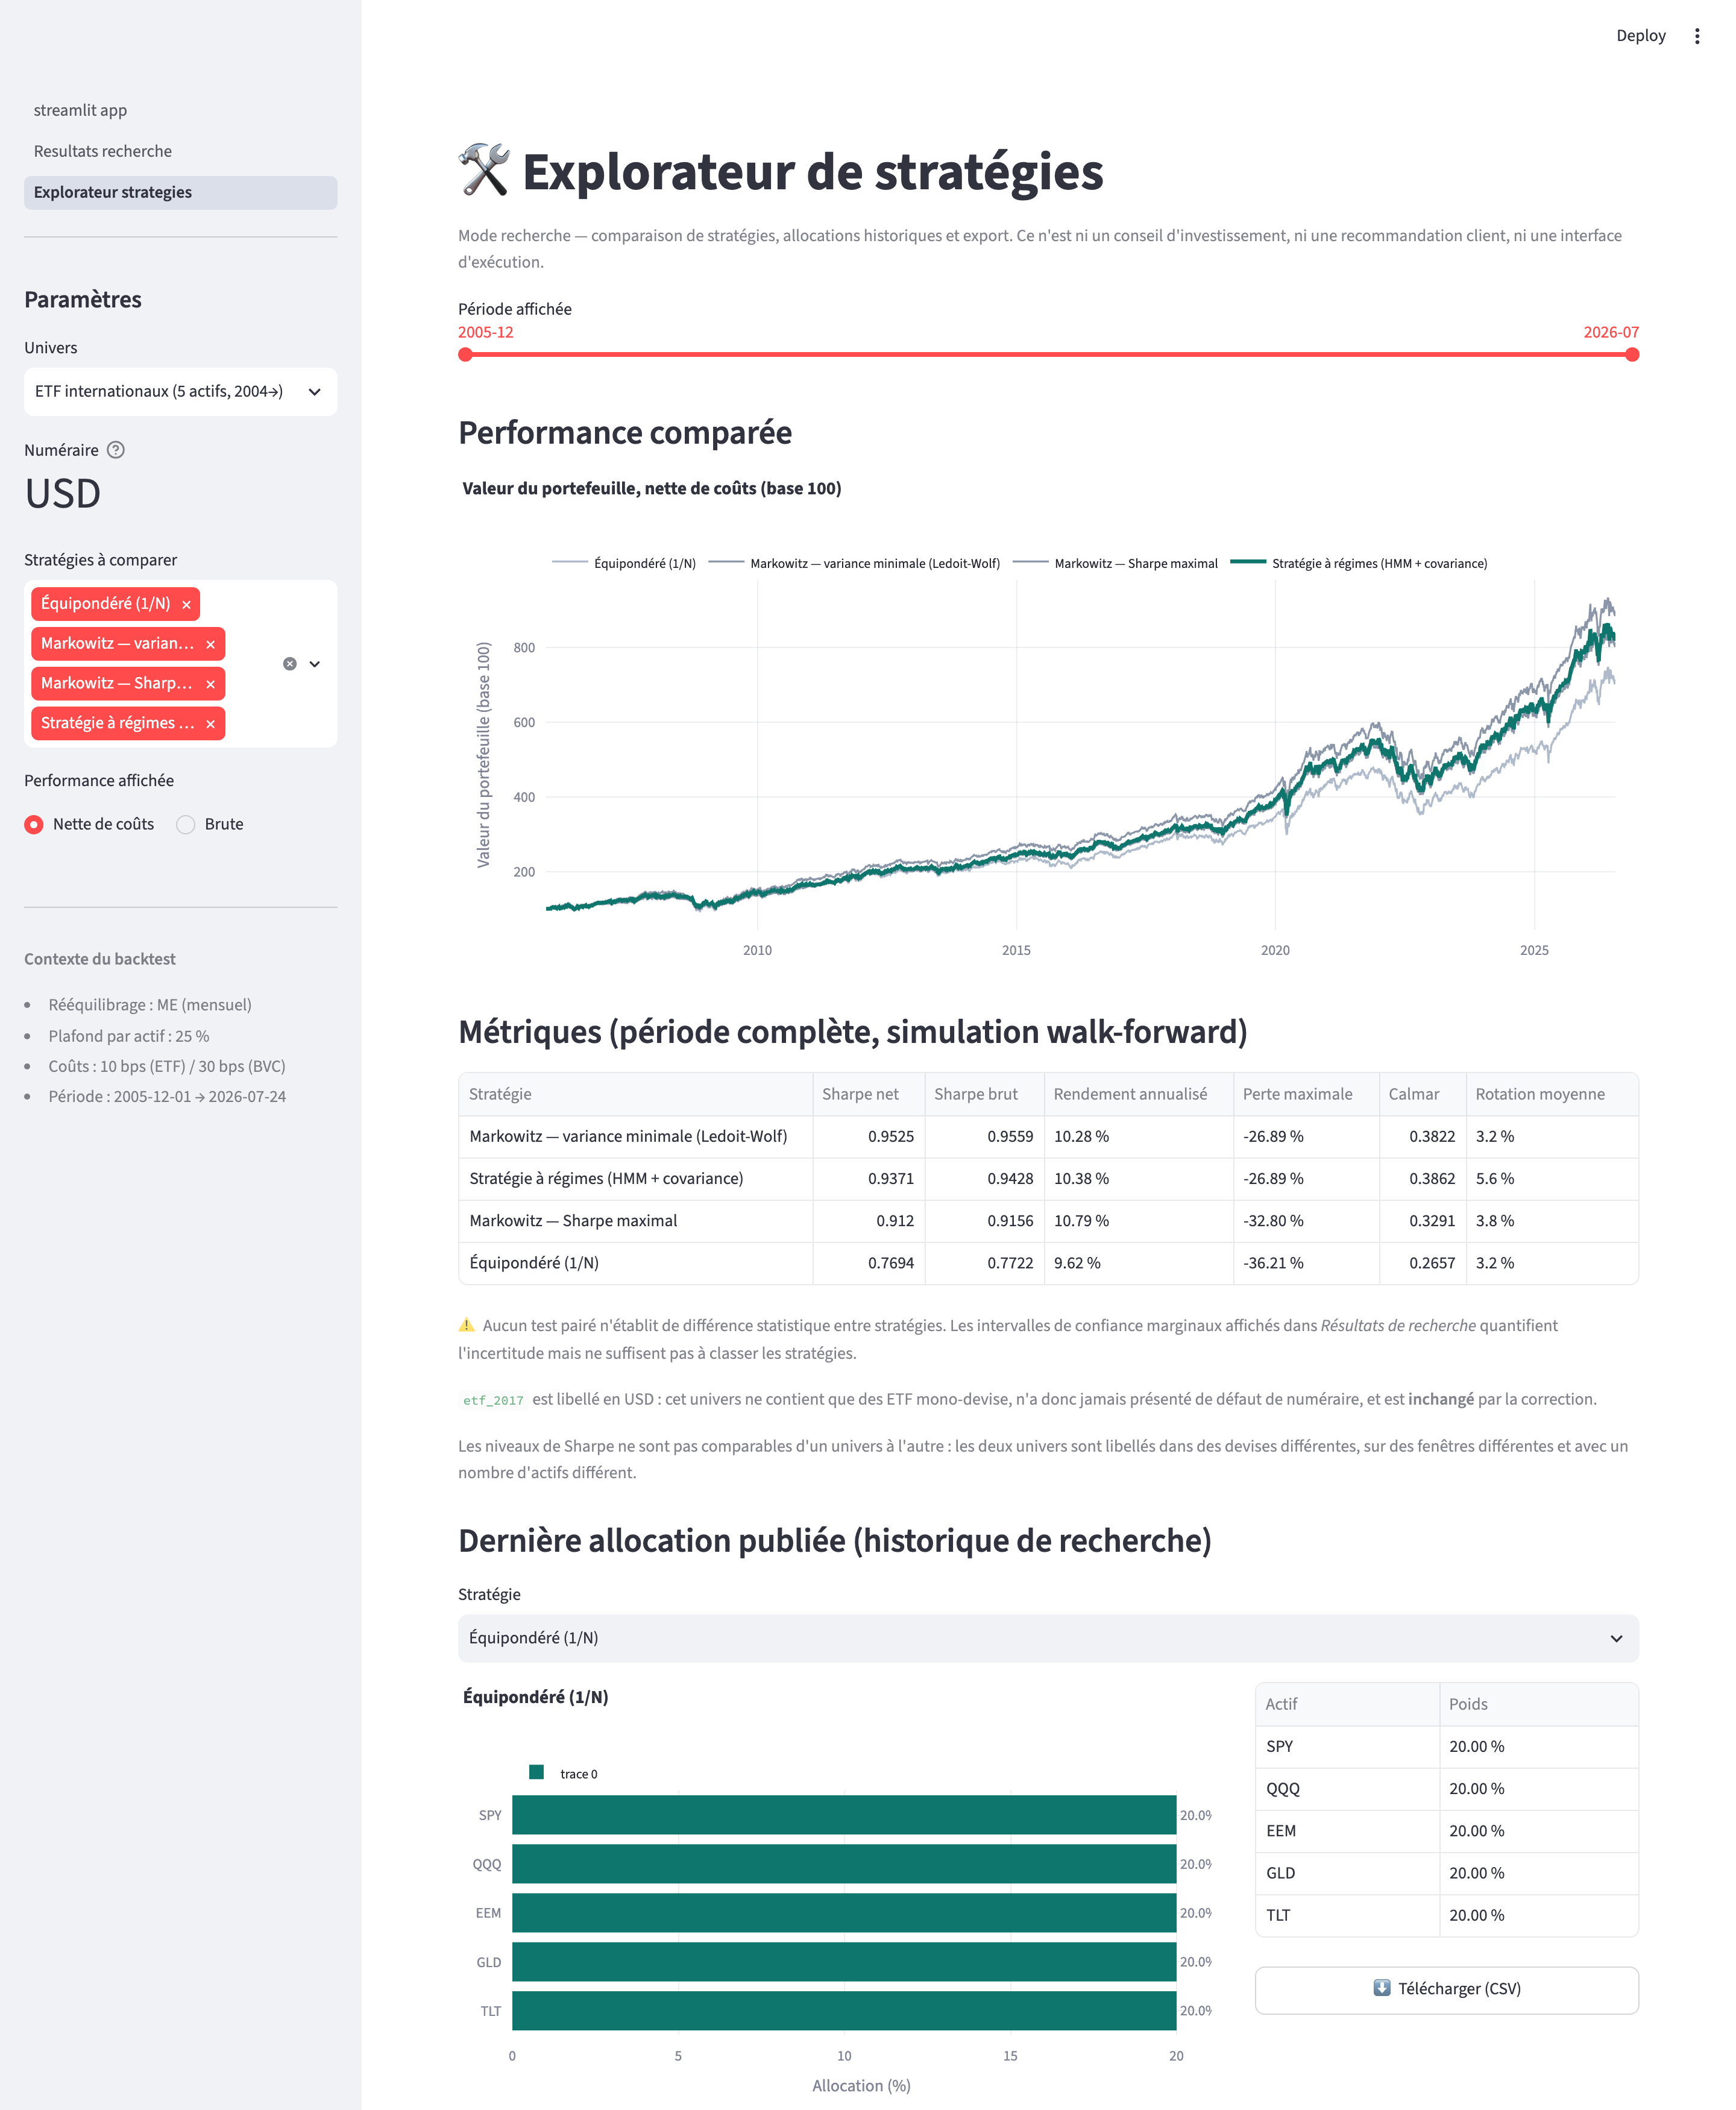
\includegraphics[width=0.94\textwidth]{assets/figures/dashboard_page2_full_01.png}
  \caption{Tableau de bord — page « Explorateur de stratégies ». Cette vue
  expose la performance, le risque, les coûts et l'allocation au lieu de réduire
  la décision à un seul ratio.}
  \label{fig:dashboard-analyste}
\end{figure}

L'interface REST offre la même information à un consommateur machine. Elle est
volontairement en lecture seule : elle sert des allocations historiques et des
explications déjà produites par la chaîne, mais n'accepte ni données de marché,
ni ordre, ni recalibrage à la demande. Chaque réponse liée à un univers rend
obligatoires la devise de base et le statut de couverture. L'absence de ces
champs serait une erreur de contrat, non une information facultative.

\begin{figure}[p]
  \centering
  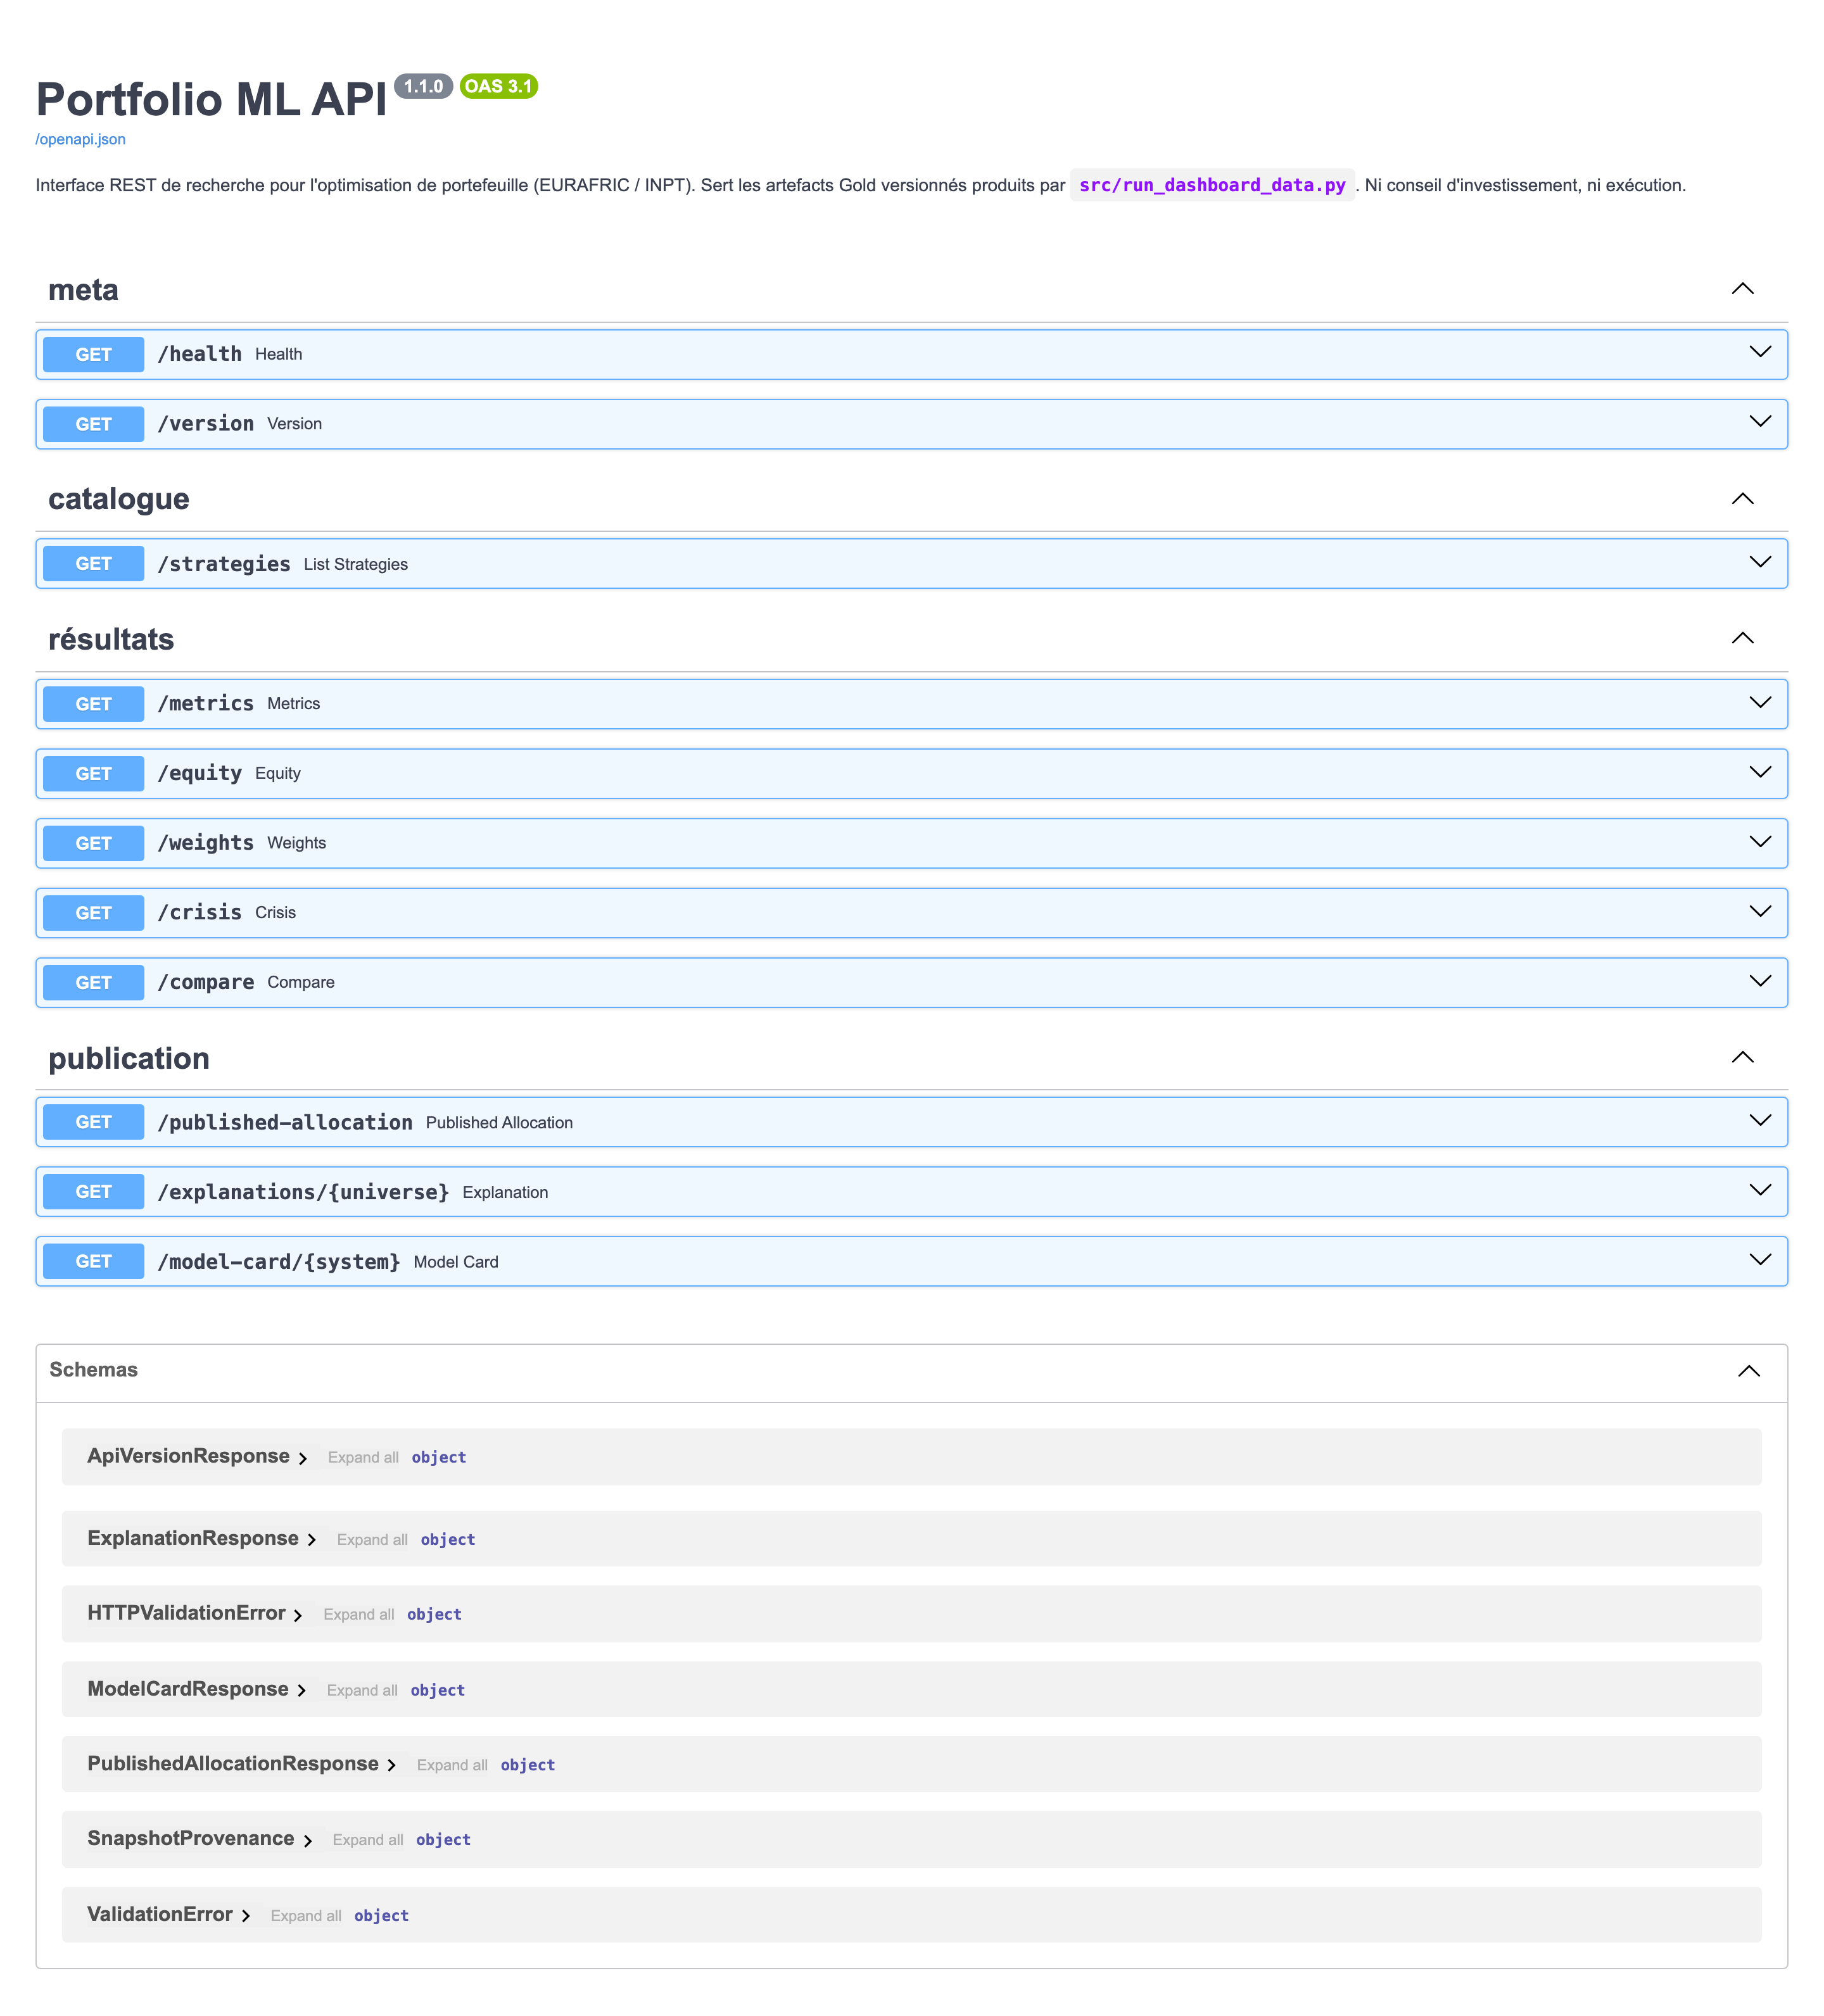
\includegraphics[width=0.94\textwidth]{assets/figures/api_swagger.png}
  \caption{Contrat OpenAPI du service de recherche en lecture seule. Les routes
  de publication exposent l'allocation historisée, son explication, sa carte de
  modèle et la provenance du snapshot ; aucune route d'ordre n'existe.}
  \label{fig:api-final}
\end{figure}

% -----------------------------------------------------------------------------
\section{Expliquer des objets différents de manière différente}
% -----------------------------------------------------------------------------

Une explication n'est pertinente que si elle porte sur la décision réellement
prise. Le système principal \texttt{regime\_conditional} ne contient ni Random
Forest ni XGBoost : lui appliquer SHAP aurait expliqué un modèle qui n'existe
pas. Deux mécanismes complémentaires ont donc été construits.

\begin{figure}[htbp]
  \centering
  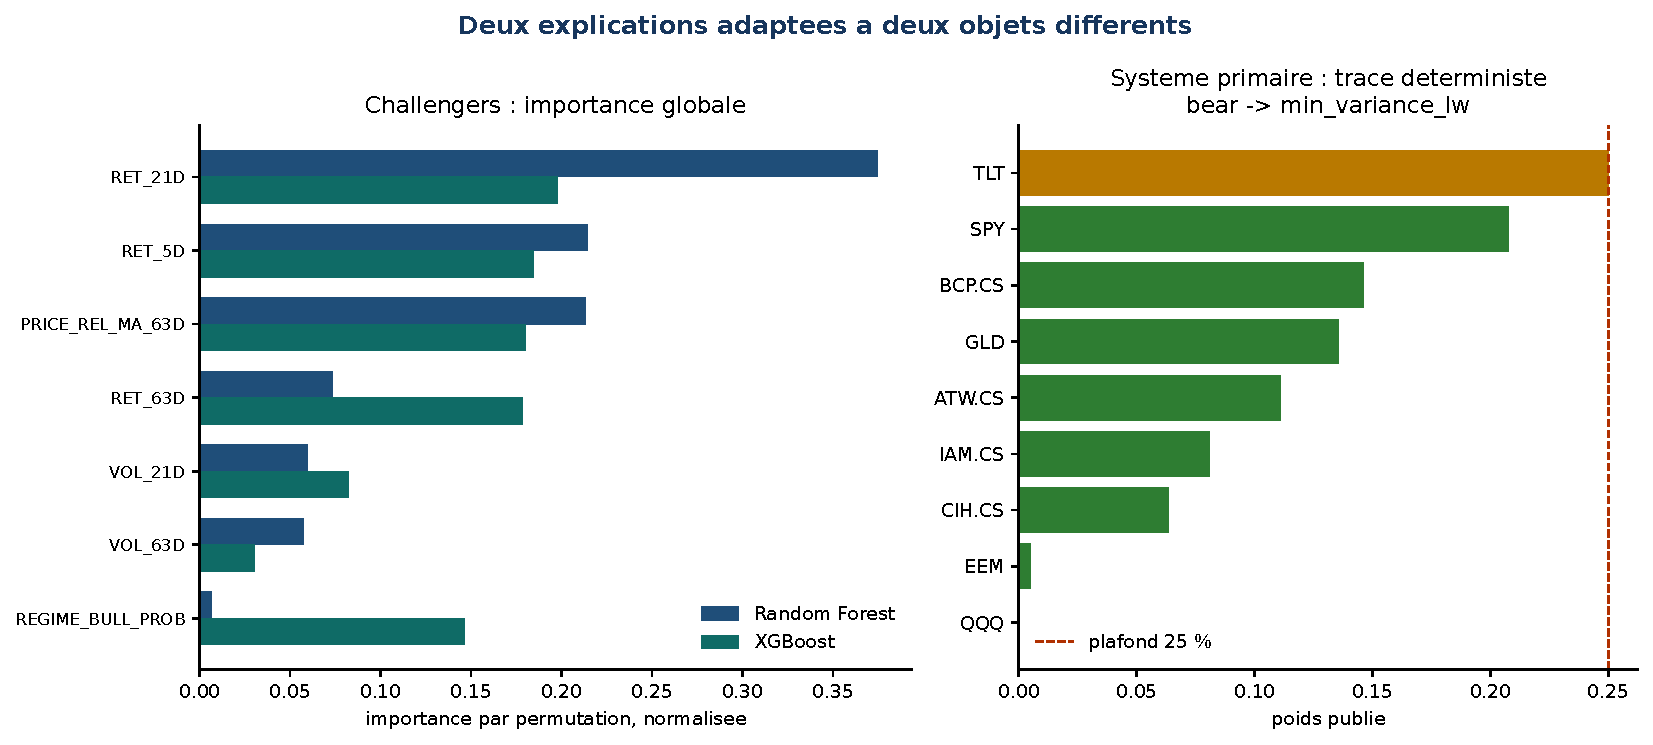
\includegraphics[width=\textwidth]{assets/figures/explicabilite.pdf}
  \caption{Explicabilité adaptée au rôle du modèle. À gauche, importances
  globales des challengers ; à droite, trace reconstructible de la décision
  finale du système à régimes sur \texttt{full\_2021}.}
  \label{fig:explicabilite-finale}
\end{figure}

\paragraph{Système à régimes.} La trace enregistre les probabilités du HMM, le
régime retenu, le sous-optimiseur choisi, la covariance utilisée, les contraintes
et les poids finaux. Sur la décision illustrée, le régime est baissier et
\texttt{min\_variance\_lw} est appelé. Quatre actifs atteignent le plafond de
25~\% et QQQ reçoit un poids nul. L'explication révèle ainsi une réalité métier :
la contrainte peut déterminer davantage l'allocation que le classement issu du
modèle.

\paragraph{Challengers arbres.} XGBoost fournit nativement les contributions
TreeSHAP ; pour Random Forest, une décomposition exacte des chemins d'arbres a
été implémentée. L'additivité est vérifiée numériquement : la somme du biais et
des contributions reconstruit chaque prédiction. Une permutation d'importance
complète cette explication locale. Ce choix évite d'ajouter une pile native
\texttt{numba}/\texttt{llvmlite} dans un environnement qui avait déjà rencontré
un conflit de bibliothèques natives.

L'explication va jusqu'au lien entre prédiction et portefeuille. Sur
\texttt{etf\_2017}, le classement RF et les poids présentent une concordance de
$-1{,}000$ : l'actif prédit premier reçoit zéro, parce que la covariance et le
plafond dominent l'optimisation. Ce résultat explique pourquoi une meilleure
prédiction n'implique pas automatiquement une meilleure stratégie.

% -----------------------------------------------------------------------------
\section{Performance économique : regarder aussi l'intensité de trading}
% -----------------------------------------------------------------------------

Le ratio de Sharpe net n'est pas seulement une propriété du signal. Il dépend de
la fréquence à laquelle le portefeuille est modifié et du coût appliqué à cette
rotation. La figure~\ref{fig:strategie-cout} replace donc les modèles sur deux
axes : performance et intensité de trading.

\begin{figure}[htbp]
  \centering
  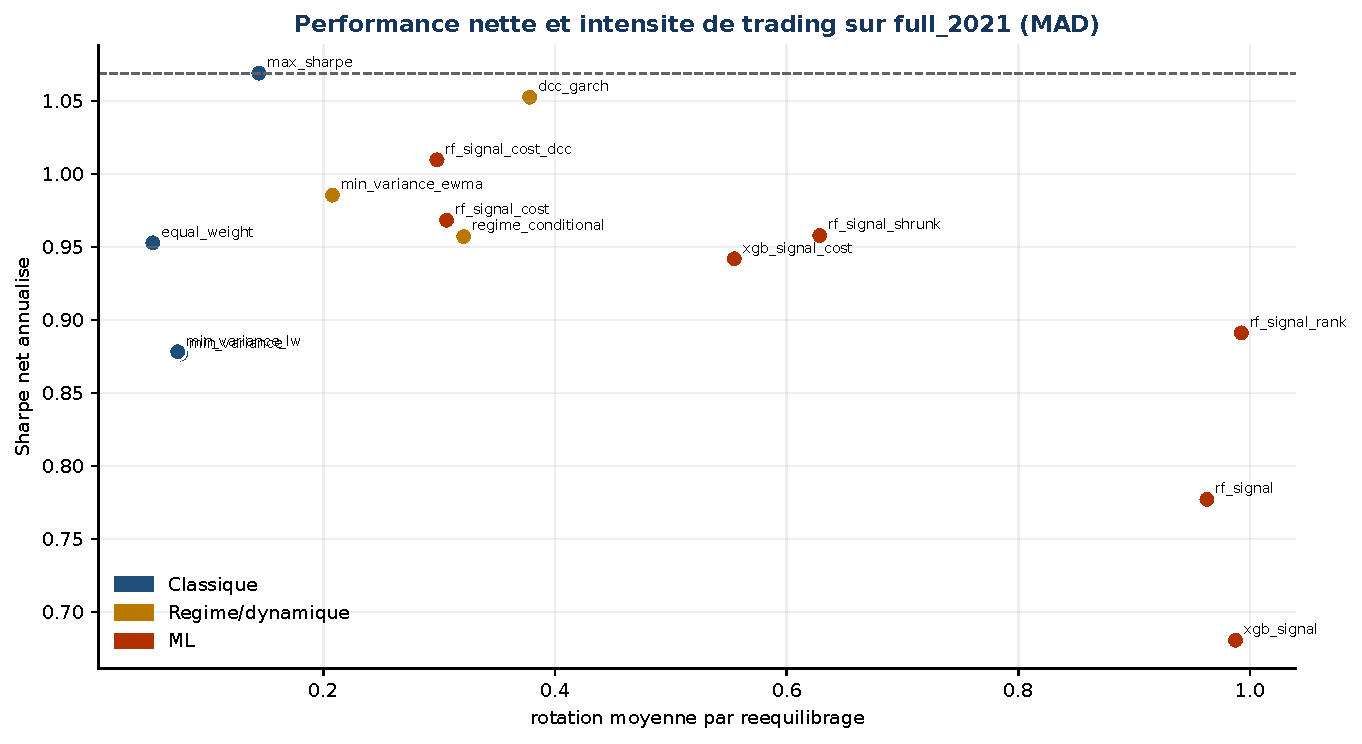
\includegraphics[width=0.93\textwidth]{assets/figures/strategie_cout.pdf}
  \caption{Sharpe net et rotation moyenne par rééquilibrage sur
  \texttt{full\_2021} en MAD. Les modèles de signal occupent généralement la
  zone la plus coûteuse sans compensation robuste en performance.}
  \label{fig:strategie-cout}
\end{figure}

Une sensibilité à 0,5$\times$, 1$\times$, 1,5$\times$ et 2$\times$ les coûts de
référence a été calculée par revalorisation du même chemin de poids sous un coût
linéaire. Elle ne constitue pas une ré-optimisation et ne modélise ni impact de
marché ni capacité. Tous les Sharpes nets ponctuels reportés restent positifs à
2$\times$ les coûts, fait descriptif qui ne démontre ni robustesse économique ni
possibilité d'exécution. L'information utile est relative : les modèles de
signal, plus actifs, sont les plus fragiles au coût.

% -----------------------------------------------------------------------------
\section{Artefacts de gouvernance}
% -----------------------------------------------------------------------------

Trois cartes de modèle sont générées depuis Gold : une carte du comparateur
primaire à régimes et une carte pour chacun des challengers RF et XGB. Elles ne
leur attribuent pas le même statut. Le premier reste le comparateur primaire
pré-spécifié pour White/SPA ; il n'est ni recommandé ni présenté comme système
de référence après observation du résultat. Les challengers sont exploratoires
et leurs attributions ne reçoivent aucune interprétation causale.

Chaque carte contient l'identité de la release, les données et fenêtres, les
contraintes, les métriques, les résultats pairés, les limites, les usages
interdits et les exigences de monitoring. Le document de gouvernance fixe en
outre les responsabilités, le processus challenger, le versionnement, le
recalibrage, le rollback et la protection des données. La ligne de validation
indépendante reste vide volontairement : l'équipe qui construit ne peut pas
s'auto-déclarer validateur indépendant.

% -----------------------------------------------------------------------------
\section{Reproductibilité et exploitation contrôlée}
% -----------------------------------------------------------------------------

\begin{figure}[htbp]
  \centering
  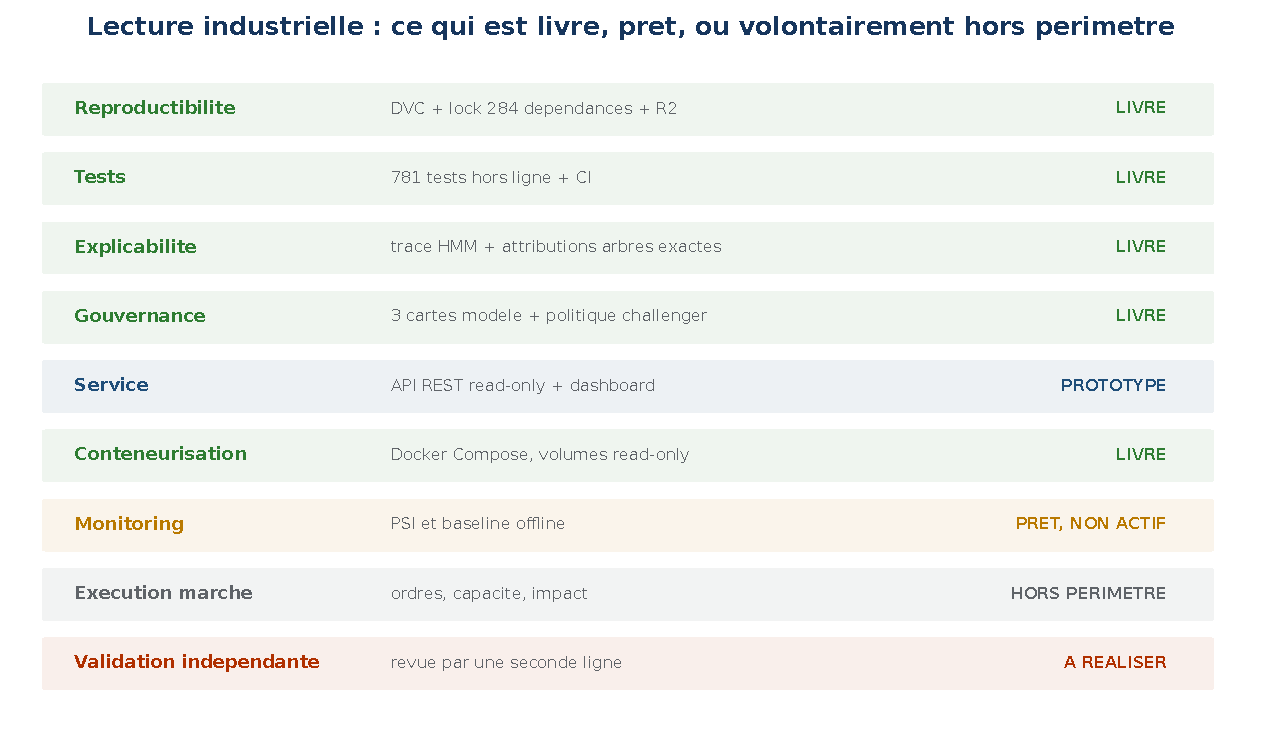
\includegraphics[width=\textwidth]{assets/figures/industrialisation.pdf}
  \caption{État industriel du livrable. « Prêt » signifie que les artefacts et
  contrôles existent ; cela ne signifie pas qu'un service est actif ou autorisé
  en production.}
  \label{fig:industrialisation}
\end{figure}

La release fige les dépendances Python dans un fichier de 284 versions, les
données et résultats avec DVC, et leur stockage distant sur un bucket R2
compatible S3. Une installation propre peut matérialiser le snapshot puis
vérifier ses empreintes. Le dépôt comprend une image Docker et une composition
de services en lecture seule. L'intégration continue exécute les contrôles qui
ne nécessitent pas les données privées de la télécommande ; les portes de
release dépendantes de Gold restent exécutées localement avant publication.

Au moment de ce rapport, \textbf{plus de 780 tests} couvrent notamment les contrats de
données, l'absence de regard vers le futur, les solveurs, les chemins de repli,
les caches, les statistiques pairées, la correction de multiplicité, les cartes
de modèle, les faits publiés et le texte du PDF rendu. Le nombre brut n'est pas
une preuve de correction ; l'intérêt est que plusieurs tests rejouent des
incidents réels et échouent si la classe d'erreur réapparaît.

\begin{figure}[p]
  \centering
  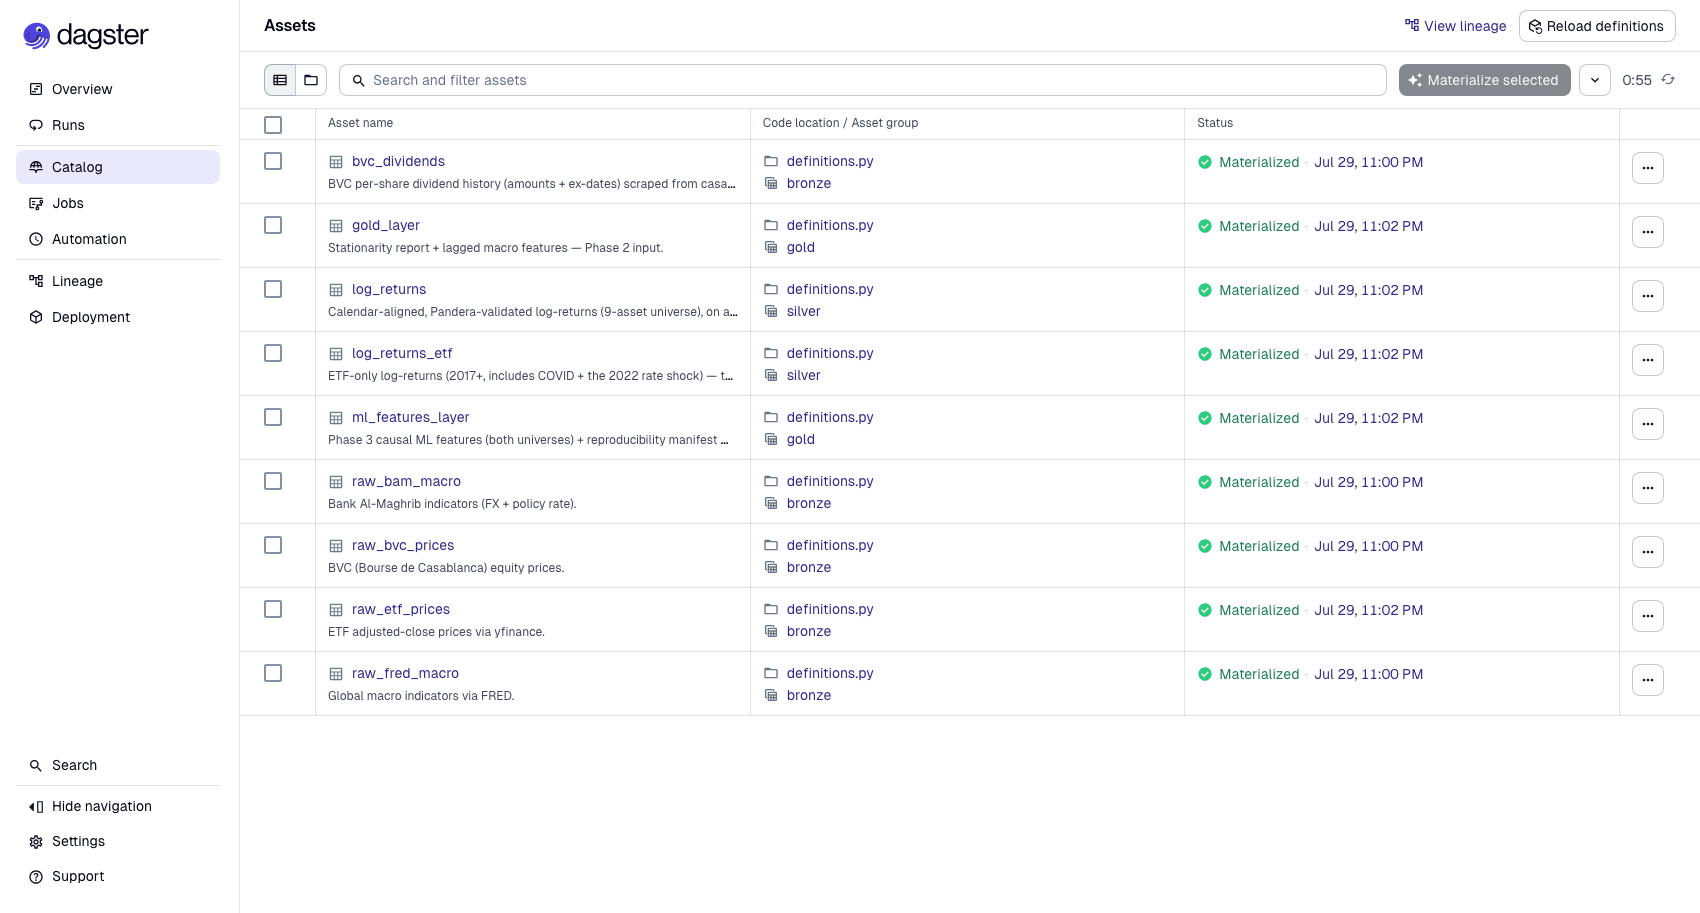
\includegraphics[width=0.95\textwidth]{assets/figures/dagster_assets.png}
  \caption{Graphe d'actifs Dagster : orchestration locale et lignage des couches
  du pipeline. L'ordonnanceur reste arrêté sur la release de soutenance.}
  \label{fig:dagster-final}
\end{figure}

% -----------------------------------------------------------------------------
\section{Monitoring prêt, mais non actif}
% -----------------------------------------------------------------------------

Le projet fournit une baseline hors ligne et des fonctions de mesure pour le
PSI des variables, la dérive des prédictions, la fréquence de régime, la
rotation, la concentration et les replis. Sans flux live, ces mesures ne doivent
pas être présentées comme un monitoring actif. L'ordonnanceur Dagster a été
arrêté après un incident où une exécution avait publié des artefacts de versions
différentes ; une relance automatique sur une release d'évaluation figée ferait
également bouger les données sous des résultats déjà publiés.

Quatre conditions précèdent toute activation : publication atomique des
artefacts, vérification du manifeste avant lecture, répertoires de release
versionnés avec verrouillage, et rollback exercé au moins une fois. La position
actuelle — \textbf{prêt, non actif} — est donc un choix de maîtrise du risque,
pas un oubli opérationnel.

% -----------------------------------------------------------------------------
\section{Notebooks : exploration sans contaminer la release}
% -----------------------------------------------------------------------------

Les notebooks historiques ont été conservés comme supports pédagogiques, mais
sécurisés : ils lisent les artefacts Gold publiés et ne reconstruisent pas la
chaîne d'évaluation lors d'une exécution interactive. Quatre notebooks de
synthèse ont été ajoutés pour la soutenance : histoire du résultat, preuve
statistique, explicabilité et risque, reproductibilité et gouvernance. Ils
servent à explorer et raconter le projet, non à fabriquer une seconde source de
vérité parallèle au pipeline.

Cette séparation répond à un risque classique des projets académiques : un
notebook permet facilement d'exécuter des cellules hors ordre, d'écraser un
résultat ou de charger un fichier local non versionné. Ici, les expériences
canoniques vivent dans des scripts, des étapes DVC et des artefacts contrôlés ;
le notebook devient une fenêtre de lecture. L'étude exploratoire sur l'historique
marocain profond (2005--2024, 12 actions) est explicitement hors release~: elle
a accru le coefficient d'information des signaux sans établir d'avantage de
portefeuille. Son intégration exigerait une source contractualisée, un
rapprochement avec la période récente, et des ajustements de dividendes et
d'opérations sur titres. Elle sert donc de résultat de recherche, pas d'entrée
silencieuse dans la chaîne canonique.

% -----------------------------------------------------------------------------
\section{Ce qui est livré, et ce qui ne l'est pas}
% -----------------------------------------------------------------------------

Le prototype offre une chaîne de recherche reproductible, des décisions
historiques expliquées, des interfaces de consultation, un paquetage, une
gouvernance et des contrôles de dérive hors ligne. Il n'offre pas l'exécution
d'ordres, la gestion de liquidité en temps réel, l'impact de marché, la capacité,
une couverture de change, une haute disponibilité ou une validation indépendante.

Cette frontière est volontairement visible dans le code, les contrats API, les
cartes de modèle et les interfaces. Elle protège le lecteur contre une confusion
fréquente : un prototype techniquement soigné n'est pas, pour autant, un modèle
autorisé à prendre une décision financière réelle.

\begin{resultatbox}{Ce qui fait ressortir le projet}
La valeur professionnelle du livrable tient à la combinaison rarement réunie
dans un PFA : données multi-sources contractualisées, moteur temporel causal,
comparaison statistique corrigée de la recherche, explicabilité adaptée à la
décision, traçabilité des replis, faits publiés générés, paquetage et limites
opérationnelles explicites. Le résultat ML est négatif ; la démonstration de ce
résultat est, elle, substantielle.
\end{resultatbox}
